\documentclass{article}
\usepackage[utf8]{inputenc}
\usepackage{enumitem}

\title{Assurance vie}
\author{Gaëtan Bouget \\ \href{mailto:bouget.g@gmail.com}{bouget.g@gmail.com}}
\date{\today}

\usepackage[french]{babel}
\usepackage{natbib}
\usepackage{graphicx}
\usepackage{xcolor}
\usepackage{mdframed}
\usepackage{lscape}
\usepackage{tcolorbox}
\usepackage[paper=portrait,pagesize]{typearea}
\usepackage[linguistics]{forest}

\usepackage{hyperref}
\usepackage{eurosym}


\definecolor{swotS}{RGB}{199,236,12}

\addtolength{\skip\footins}{2pc plus 5pt} % espace des notes de fin page

\newcommand{\blackFrame}[2]{
    \begin{tcolorbox}[colback=white,colframe=black!100!white,title={#1}]
        #2
    \end{tcolorbox}
}

\begin{document}

\maketitle
\thispagestyle{empty}

\vspace{3cm}

\begin{center}
    
\includegraphics[width=5cm]{resources/dandelion.jpg}
\end{center}

\vspace{3cm}

Titulaire d'un master en informatique, je travaille depuis deux ans à Gfi Informatique dans la branche fonctionnelle de la Banque, Finance et Assurance. Parmi nos nombreux clients, j'interviens pour le compte de Cardif, filiale du groupe BNP Paribas, dans l'exploitation et l'évolution de son système d'information.

\newpage

\tableofcontents

\newpage

%% --------------------------------------------------------------
%% --------------------------------------------------------------
\section{Généralités sur l'assurance}

\subsection{Pourquoi s'assurer ?}
Le rôle de l'assurance est d'apporter une sécurité face aux dangers de la vie. Dans le contexte socio-économique actuel, l'être humain redoute la survenance de divers évènements comme : la panne de voiture, la coupure d'électricité, l'incendie domestique, le décès d'un proche, etc. Ces événements dont le caractère est aléatoire et redouté sont appelés risques. Dans le lexique des assurances, un risque qui se réalise est appelé sinistre.

Pour se protéger d'un risque, une personne peut conclure un contrat d'assurance avec un assureur. En contrepartie du paiement d'une prime, l'assureur s'engage à verser une prestation (somme d'argent souvent) si un sinistre se produit.

\subsection{Qui sont les principaux acteurs ?}
\subsubsection{Assureur}
L'assureur est une personne morale qui s'engage à verser une prestation (financière généralement) lorsque l'assuré est victime d'un sinistre. En France, l'exercice des opérations d'assurances nécessite obligatoirement un agrément auprès de l'Autorité de Contrôle Prudentiel et de Résolution (ACPR, L321-1). L'organisme d'assurances peut revêtir trois formes juridiques (L310-1) :
\begin{itemize}
    \item Les sociétés d'assurances (réglementées par le code des assurances) :  société anonyme, société d'assurance mutuelle ou société européenne (L322-1)
    \item Les mutuelles (réglementées par le code de la mutualité)
    \item Les instituts de prévoyance (réglementés par le code de la sécurité sociale)
\end{itemize}

À titre indicatif, le registre géré par l'ACPR permet de connaitre la liste de tous les organismes agréés. Cependant, dans la pratique, la souscription d'un contrat d'assurance se conclut rarement avec l'assureur directement, mais plutôt par le biais d'un intermédiaire, appelé distributeur d'assurances.

\subsubsection{Distributeur}
Régie par le livre 5 du code des assurances, l'activité de distribution consiste à \textit{fournir des recommandations sur des contrats d'assurance [...], à présenter, proposer ou aider à conclure ces contrats ou à réaliser d'autres travaux préparatoires à leur conclusion, ou à contribuer à leur gestion et à leur exécution, notamment en cas de sinistre} (L511-1).

Historiquement, le mode de distribution la plus courante --~si ce n'est l'unique~-- est l'intermédiation : c'est-à-dire la mise en relation du \textit{client} (personne souhaitant souscrire ou adhérer à un contrat d'assurance) avec l'assureur. Profession strictement encadrée par l'État, l'intermédiaire a l'obligation de s'inscrire dans le registre ORIAS dont la lecture est accessible à tous les citoyens (L512-1). Les principaux statuts juridiques des intermédiaires sont :

\begin{itemize}
    \item Courtier
    \item Agent général d'assurances
    \item Mandataire d'assurances
    \item Mandataire intermédiaire d'assurances
\end{itemize}

Depuis quelques décennies, de nouveaux modes de distribution émergent et bousculent le marché traditionnellement régi par les intermédiaires. Ainsi, en 1970, le rapprochement entre le secteur bancaire et le secteur des assurances donne naissance à la notion de \textit{bancassurance} dont les parts de marché ne cessent de croitre. D'ailleurs, je suppose que c'est dans cette logique que la Directive sur la Distribution d'Assurance (DDA) adoptée en 2016 abroge l'ancienne directive sur les intermédiaires. Dorénavant, sur le plan terminologique, la distribution englobe la notion d'intermédiation même si les termes restent flous dans certains textes selon Jean Bigot\footnote{DDA et les mots des technocrates
[en ligne]. [consulté le 24 décembre 2019]. Disponible sur : \href{https://www.argusdelassurance.com/juriscope/decryptages/dda-et-les-mots-des-technocrates.145990}{https://www.argusdelassurance.com/.../dda-et-les-mots-des-technocrates}}.

Pour finir, les \textit{assurances affinitaires} peuvent être proposées par des distributeurs dont le coeur de métier est très éloigné de l'assurance. La Fédération des garanties et assurances affinitaires (FG2A) définit une assurance affinitaire comme \textit{toute garantie d'assurance, d'assistance ou service accessoire en lien avec l'univers d'un produit ou service distribué par un distributeur non-assureur et qui n'est pas le motif principal d'achat du client}.

\subsubsection{Souscripteur}
Le souscripteur est une personne morale ou physique dont le rôle est d'établir et de conclure le contrat avec l'assureur. Il est redevable du paiement des primes sauf dans le cas des contrats de groupe où le règlement peut incomber à l'adhérent (L141-2, L141-3).

\blackFrame{Votum mortis}{
    Un contractant ne peut pas conclure une assurance en cas de décès sur la tête d'une tierce personne sans obtenir son consentement par écrit (L132-2). De même, l'article L132-3 prohibe toute assurance en cas de décès sur la tête d'un mineur âgé de moins de douze ans, d'un majeur en tutelle ou d'une personne placée dans un établissement psychiatrique d'hospitalisation.
}

\subsubsection{Adhérent}
Dans le cas des contrats collectifs, la souscription est réalisée par une personne morale ou un chef d'entreprise au profit des membres d'une même collectivité, appelés adhérents (L141-1). Elle repose sur une relation tripartite :
\begin{enumerate}
    \item Le souscripteur et l'assureur conclut un contrat cadre pour fixer les conditions d'application du contrat aux futurs adhérents.
    \item Le futur adhérent remet un bulletin d'adhésion à l'assureur pour la création d'un contrat individuel lié au contrat de groupe.
\end{enumerate}

\subsubsection{Assuré}
L'assuré désigne la personne sur laquelle porte le risque. En cas de sinistre, l'assuré reçoit la prestation sauf dans l'assurance en cas de décès où il s'agit du bénéficiaire.

\subsubsection{Bénéficiaire}
L'assurance en cas de décès de l'assuré prévoit le versement de la prestation à un ou plusieurs bénéficiaires désignés dans la police par le contractant (souscripteur ou adhérent).

Suite à l'acceptation du bénéfice par le bénéficiaire en assurance sur la vie (contrat rachetable), le contractant ne peut plus le révoquer ni disposer de l'argent versé sur le contrat (rachat, avance ou nantissement) sans obtenir l'accord du bénéficiaire au préalable (L132-9).

\subsection{Comment souscrire un contrat ?}
La souscription d'un contrat s'effectue auprès d'un organisme d'assurances. Le cycle peut être découpé en trois étapes :
\begin{enumerate}
    \item Définir les besoins pour déterminer le contrat d'assurance adapté
    \item Jauger l'état du marché : comparateur d'assurances, intermédiaires, etc.
    \item Conclure la vente par la signature de la police d'assurance sur un support durable
\end{enumerate}

\subsection{Que se passe-t-il après la souscription du contrat ?}
Les possibilités dépendent de l'accord passé avec l'assureur (dont le récapitulatif figure dans la police d'assurance). Néanmoins, le mode de gestion de l'argent par l'assureur détermine en grande partie les actions possibles pendant la vie du contrat. L'assureur dispose de deux possibilités pour gérer les primes (c'est-à-dire l'argent versé par les clients) :

\begin{itemize}
    \item la gestion par mutualisation dans la majorité des cas ;
    \item la gestion par capitalisation dans le cadre de l'assurance sur la vie.
\end{itemize}

\subsubsection{Gestion par mutualisation}
Dans la gestion d'un contrat par mutualisation (cf figure~\ref{gestion_mutualisation} page~\pageref{gestion_mutualisation}), l'argent versé par le contractant sur le contrat est utilisé pour indemniser les autres contrats du même type. Pour ce faire, les versements de chaque client s'accumulent dans un fonds commun. Puis, en cas de sinistre de l'un d'entre-eux, l'assureur retire l'argent du fonds commun pour effectuer l'indemnisation. Pour le client, le système fonctionne à perte dans le sens où il ne peut pas récupérer volontairement l'argent qu'il a versé à l'assureur. Cependant, l'avantage est de se couvrir d'un risque à un coût relativement peu coûteux par rapport au montant de l'indemnité perçue en cas de sinistre. Côté assureur, l'actuariat joue un rôle primordial dans l'analyse de l'impact financier du risque afin de concilier deux tableaux : proposer des tarifs compétitifs au client tout en préservant les marges de l'assureur.

\begin{figure}[h!]
    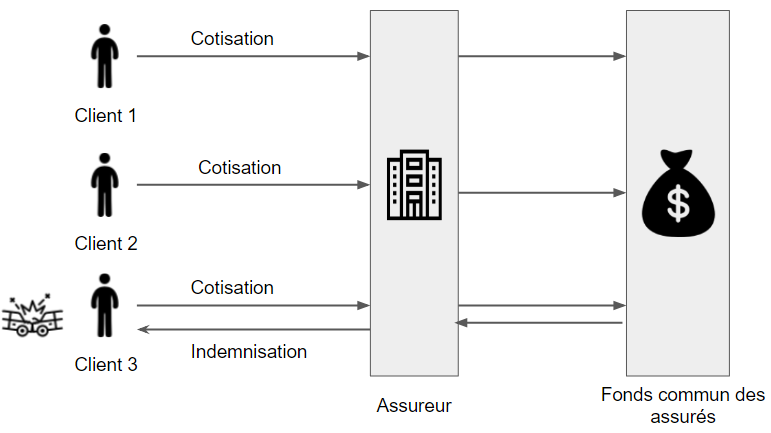
\includegraphics[width=\textwidth]{resources/gestion_mutualisation.PNG}
    \caption{
        \label{gestion_mutualisation} Gestion par mutualisation
    }
\end{figure}

\subsubsection{Gestion par capitalisation}
Dans la gestion par capitalisation (cf figure~\ref{gestion_capitalisation} page~\pageref{gestion_capitalisation}), l'argent versé par le client (contractant) s'accumule sur son propre contrat. Ensuite, l'assureur investit cet argent sur des supports financiers pour le faire fructifier. Contrairement à la gestion par mutualisation, le contractant possède un droit de créance sur les sommes versées sur le contrat.

Sauf cas contraires (bénéficiaire acceptant, nantissement, etc.), le contractant peut débloquer l'argent versé sur contrat à tout moment grâce à une demande de rachat. Dès lors, l'assureur verse tout ou partie du capital présent sur le contrat additionné des éventuelles plus-values (également appelées intérêts ou produits) réalisées grâce aux placements sur les supports financiers. En moyenne, la durée d'attente entre la demande de rachat et la réception du paiement est de l'ordre de quelques semaines.

\begin{figure}[h!]
    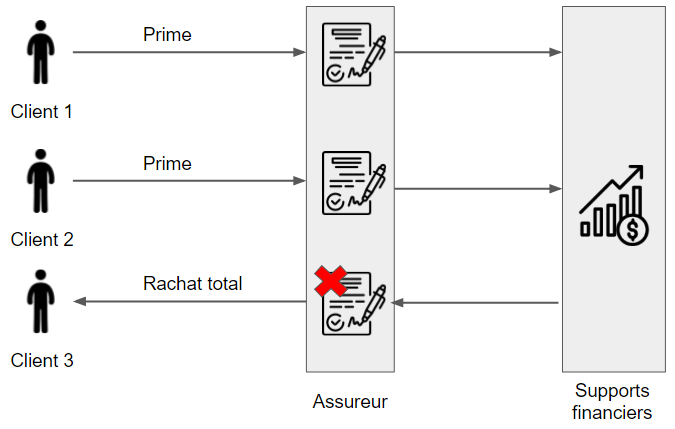
\includegraphics[width=\textwidth]{resources/gestion_capitalisation.PNG}
    \caption{\label{gestion_capitalisation} Gestion par capitalisation
    }
\end{figure}

\blackFrame{Résumé}{
La gestion par capitalisation (assurance en cas de vie) est adaptée aux \textbf{produits d'épargne} alors que la gestion par mutualisation (toutes les autres assurances : assurances habitation, automobile, maladie, décès, etc.) est utilisée pour les \textbf{produits de prévoyance}.
}

\subsection{Comment dénouer le contrat ?}
Le dénouement du contrat peut être consécutif à un sinistre ou à échéance du contrat. En assurance sur la vie (gestion par capitalisation), le client peut clore le contrat de sa propre initiative suite à un rachat total.  

% TODO : Aborder la résiliation ?

\subsection{Comment classer les assurances ?}
Les assurances peuvent être classées de plusieurs manières en fonction :
\begin{itemize}
    \item de la branche d'après l'article R321-1 pour l'octroi de l'agrément d'exercice ;
    \item de la nature du risque : assurances de dommages ou assurances de personnes ;
    \item du mode de gestion des primes par l'assureur : mutualisation ou capitalisation ;
    \item du type de la prestation fournie : principe forfaitaire ou principe indemnitaire.
\end{itemize}

La classification habituelle des assurances figure en annexe \ref{appendix:classification-assurances}.

\subsubsection{Classification selon la nature du risque}
La classification selon la nature du risque distingue deux catégories : les assurances de dommages et les assurances de personnes. Les assurances de dommages couvrent le patrimoine de l'assuré alors que les assurances de personnes portent sur sa santé (en vie et en bonne santé physique et mentale).

Exemples :
\begin{itemize}
    \item Assurances de dommages : assurance habitation, assurance voiture, assurance responsabilité civile, etc.
    \item Assurances de personnes : assurance maladie, assurance en cas de vie, assurance en cas de décès, etc.
\end{itemize}

\subsubsection{Classification selon le mode de gestion des primes}
L'assurance en cas de vie est la seule assurance gérée en capitalisation par l'assureur. Cela signifie que l'argent versé sur le contrat est investi par l'assureur sur les marchés financiers. En revanche, lorsque la gestion est faite en mutualisation, alors les primes servent à indemniser les sinistres du même type et ayant eu lieu la même année.

\subsubsection{Classification selon le type de prestation fournie}
Sous cet angle, le critère de discrimination est basé sur le montant de l'indemnisation perçue par l'assuré. Tout d'abord, le type indemnitaire couvre l'assuré en versant une indemnité dont le montant ne peut excéder la valeur de la \textit{chose} sinistrée au moment de l'accident. Ainsi, une expertise peut parfois s'avérer nécessaire pour estimer cette valeur. À contrario, si le contrat repose sur le type forfaitaire, alors le montant est clairement explicité dès la souscription du contrat sans tenir compte du montant du préjudice réellement subi.

La législation considère que les assurances de personnes relèvent du principe forfaitaire (L131-1) alors que les assurances de dommages se basent sur le principe indemnitaire (L121-1).

\blackFrame{Exemple}{
Après un accident, le conducteur est indemne mais la voiture est inutilisable. L'achat a été réalisé il y a cinq ans pour un montant de 15 000 euros.
\begin{itemize}
    \item Si le propriétaire a souscrit une assurance basée sur le type indemnitaire, une expertise technique peut être nécessaire pour déterminer la valeur d'achat de la \textit{chose} -- la voiture en l'occurrence -- au moment de l'accident (et non au moment de l'achat). En se basant sur plusieurs critères comme la valeur d'achat et l'état du marché, l'expertise estime le prix de la voiture au moment de l'accident. Pour cet exemple, la valeur estimée de la voiture au moment du sinistre est de 7 500 euros. Ainsi, l'indemnité perçue par l'assuré (le propriétaire de la voiture) ne peut pas excéder 7~500 euros.
    \item Si le propriétaire a souscrit une assurance basée sur le type forfaitaire, alors le montant est déterminé au moment de la souscription. Dès lors, il est possible d'imaginer plusieurs scénarios. L'un d'entre eux pourrait prévoir une indemnisation à la hauteur du prix d'achat si la voiture est inutilisable après un sinistre (donc 15~000 euros). Mais, il est tout fait possible de négocier à la hausse comme à la baisse ce montant. Bien sûr, le montant des primes à payer à l'assureur va fluctuer en même temps que le montant de la prestation perçue par l'assuré (indemnité) : le coût de la prime à payer croit avec le montant de l'indemnité perçue en cas de sinistre.
\end{itemize}
En synthèse, le principe forfaitaire peut enrichir l'assuré en cas de sinistre contrairement au principe indemnitaire. Pour rappel, l'assurance est fondée sur le caractère imprévisible et non souhaité du sinistre par l'assuré. Si ce dernier provoque intentionnellement la survenance du sinistre, alors c'est une fraude à l'assurance (reconnue comme un délit par le code pénal).
}

%% --------------------------------------------------------------
%% --------------------------------------------------------------
\newpage

\section{Fonctionnement de l'assurance vie}
L'assurance vie est fondée sur l'aléa lié à la durée de vie humaine. D'un point de vue strict, il existe deux grandes formes d'assurance vie :
\begin{itemize}
    \item Assurance en cas de décès : versement d'une prestation (capital ou rente) aux bénéficiaires désignés par le contractant si l'assuré décède avant le terme (date définie ou vie entière).
    \item Assurance en cas de vie : versement d'une prestation (capital ou rente) au contractant si l'assuré est en vie au terme du contrat. En cas de décès avant le terme, les capitaux sont conservés par l'assureur.
\end{itemize}

L'assurance en cas de décès permet de protéger les proches de l'assuré alors que l'assurance en cas de vie est utilisée comme un placement. Pour répondre simultanément à ces deux besoins, les assureurs peuvent proposer une contre assurance pour couvrir le deuxième cas ou vendre directement une assurance mixte en cas de vie et de décès. L'assurance mixte est une assurance en cas de vie avec l'adjonction d'une clause pour garantir le versement du capital à des bénéficiaires si le décès survient avant le terme (appelée clause bénéficiaire).

Dans la suite du document, l'assurance vie est vue comme une assurance mixte.

\subsection{Pourquoi souscrire un contrat d'assurance vie ?}
L'assurance vie (en cas de vie et en cas de décès) est un produit d'épargne qui permet de répondre à plusieurs objectifs grâce à un régime juridique et fiscal spécifique :
\begin{itemize}
    \item Constituer et valoriser un capital grâce aux placements sur les supports financiers.
    \item Préparer sa retraite grâce à la récupération progressive du capital (rachats partiels programmés) ou en transformant le capital en rente viagère. 
    \item Transmettre un capital en profitant des avantages fiscaux.
    \item Faire face à un besoin d'argent inopiné grâce à un capital disponible à tout moment (rachat ou avance). En moyenne, le délai d'attente entre la demande de récupération des liquidités et la réception des fonds est de quelques semaines.
\end{itemize}

\subsection{Comment fonctionne un contrat d'assurance vie ?}
Le fonctionnement d'un contrat d'assurance vie peut se résumer en quelques opérations :
\begin{itemize}
    \item Choisir les supports financiers sur lesquels investir
    \item Ajouter de l'argent
    \item Retirer de l'argent
\end{itemize}
L'arbitrage est une opération qui permet de modifier la répartition de l'épargne sur les produits financiers.

% image
\subsection{Quels sont les supports financiers ?}
L'assureur peut être perçu comme un intermédiaire entre les instruments financiers et l'investisseur (également appelé contractant ou client en fonction du contexte). L'essentiel à retenir est que l'assureur propose la détention d'instruments financiers (actifs) à travers :
\begin{itemize}
    \item Les fonds
        \begin{itemize}
            \item Les fonds en euro
            \item Les fonds diversifiés
        \end{itemize}
    \item Les unités de compte
\end{itemize}

Les fonds sont constitués d'un ensemble d'instruments financiers gérés par l'assureur. Dans le fonds en euro, l'assureur place l'argent sur des actifs peu risqués afin d'honorer deux caractéristiques clefs du fonds : la garantie du capital et la garantie cliquet (chaque année, les gains réalisés sont définitivement acquis et intègrent le capital pour produire à leur tour des intérêts). Dans un fonds diversifié, le portefeuille est constitué de plusieurs classes d'actifs différentes afin de répondre à deux problématiques : compenser une éventuelle forte baisse de prix d'une classe d'actifs et améliorer le rendement de son portefeuille.

À contrario, les unités de compte sont des supports financiers où le contractant détient \textit{directement} des titres financiers. Dans ce cas, l'assureur est tenu d'en garantir le nombre, mais la valeur d'un titre peut fluctuer à la hausse ou à la baisse.

% Approfondir le fonds diversifié (voire eurocroissance ?)
% https://www.linkedin.com/pulse/actionnariat-en-france-agissons-durgence-pour-la-pierre-de-villeneuve?articleId=6209471063114424320#comments-6209471063114424320&trk=public_profile_article_view
% https://www.linkedin.com/pulse/leurocroissance-linnovation-dans-lassurance-vie-pierre-de-villeneuve?articleId=6011078725259522048#comments-6011078725259522048&trk=public_profile_article_view

\subsection{Quels sont les types de contrats ?}
L'assurance vie se décline en deux grands types : l'assurance vie monosupport et l'assurance vie multisupport. Les primes d'un contrat monosupport sont investies dans un seul support : le fonds en euro souvent. Or, les caractéristiques du fonds en euro que sont la garantie du capital et l'effet cliquet contraignent l'assureur à orienter les primes vers des instruments financiers à faibles risques comme les obligations d'États. Depuis quelques années, les États bien notés (réputés peu risqués) empruntent à des taux très bas, ce qui se répercutent sur le rendement des investisseurs. Pour y remédier, la tendance est plutôt à la diversification des placements grâce aux contrats multisupports : une partie sur le fonds en euro pour la sécurité, et une autre partie sur les unités de compte pour rechercher la performance (rentabilité). Les pouvoirs publics encouragent d'ailleurs cette pratique en permettant le transfert des capitaux d'un contrat monosupport vers un contrat multisupport sans perdre l'antériorité fiscale du contrat d'origine.

% Contrats dérivés
% Eurocroissance : multisupport
% vie génération : monosupport en UC
% DSK / NSK : multisupport

% amendement Fourgous
\blackFrame{Amendement Fourgous}{
Dans le cadre de la loi du 26 juillet 2005 pour la confiance et la modernisation de l'économie, l'amendement Fourgous permet au souscripteur de transférer le capital d'un contrat monosupport vers un contrat multisupport sans perdre les avantages fiscaux du contrat d'origine (l'antériorité fiscale du contrat monosupport est conservée).
}

\subsection{Comment gérer l'épargne ?}
\subsubsection{Comment déposer de l'argent ?}
Le versement d'argent sur le contrat s'appelle une prime. À minima, un versement est réalisé lors de l'ouverture du contrat à la souscription. Par la suite, le contractant peut verser de l'argent à tout moment (versement libre) ou automatiser le versement des primes à des échéances régulières (primes programmées).

\subsubsection{Comment retirer de l'argent ?}
Le retrait de l'épargne est possible grâce à l'opération de rachat ou l'avance. Le rachat peut être total ou partiel. S'il est total, alors le contrat se dénoue et le contractant récupère la totalité du capital. Si le rachat est partiel, le contractant choisit le montant à retirer et éventuellement les supports à désinvestir. Dans ce cas, le contrat n'est pas dénoué et le reste du capital continue de générer des intérêts. Pour terminer, l'assureur peut également accorder une avance. Le fonctionnement d'une avance est similaire à un prêt : l'assureur prête de l'argent sans l'imputer au capital du contrat contrairement à un rachat. Bien que l'avance comporte des frais et un taux d'intérêt (débiteur pour le contractant), la solution peut parfois s'avérer moins coûteuse car la totalité du capital présent sur le contrat continue de produire des intérêts (créditeurs pour le contractant).

\blackFrame{Cas particuliers}{
    Certaines situations peuvent empêcher le contractant d'effectuer un rachat ou une avance comme le nantissement (délégation de créance). De même, depuis le 18 décembre 2007, le consentement du bénéficiaire est nécessaire si celui-ci a accepté de recevoir le capital en cas de décès.
}

\subsubsection{À quoi sert l'arbitrage ?}
La difficulté de l'investissement réside dans l'allocation d'actifs. Pour un investisseur rationnel, le rendement est la rémunération du risque. En d'autres termes, un investisseur accepte de s'exposer davantage au risque de perdre son capital en contrepartie d'un meilleur rendement (une prime de risque). Inversement, un investisseur qui souhaite améliorer le rendement de son portefeuille doit accepter de prendre des risques. C'est pourquoi le choix des supports financiers est une étape primordiale car il détermine l'ampleur des gains ou des pertes.

\blackFrame{Mandat de gestion}{
Le contractant peut mandater une tierce personne pour gérer la répartition de son épargne sur les supports financiers. La gestion sous mandat implique une première phase d'étude pour établir le profil d'investisseur afin d'ajuster au mieux le compromis entre la prise de risque et le rendement. Le mandataire peut être un spécialiste de la gestion d'actifs ou un algorithme.
}

\subsection{Comment dénouer le contrat ?}
\subsubsection{Dénouement en cas de vie}
Le dénouement d'un contrat en cas de vie de l'assuré peut avoir lieu à l'échéance du contrat ou suite à une demande de rachat total par le contactant. Dans les deux cas, les fonds sont versés au contractant.

La sortie du contrat peut s'effectuer par le versement du capital ou par une rente. Dans le cas d'une sortie en capital, l'encours du contrat peut être réglé en une seule fois (rachat total) ou échelonné sur plusieurs échéances  jusqu'à épuisement du capital (rachats partiels programmés, opération annulable). Dans une sortie en rente viagère, l'assureur conserve le capital mais s'engage à verser une rente à vie au contractant. Le montant des arrérages est en fonction de l'âge du contractant au moment du dénouement, de la date et valeur de rachat du contrat, du taux technique ainsi que des éventuelles options choisies (réversion, annuités gratuites ou garantie dépendance).

\subsubsection{Dénouement en cas de décès}
Le dénouement d'un contrat suite au décès de l'assuré est déclenché lorsque l'assureur en a connaissance suite à la réception de l'acte de décès ou lors de la consultation du répertoire national d'identification des personnes physiques (RNIPP).

% RNIPP envoie un acte de décès ?

Malgré le décès, l'assurance vie échappe à la succession de l'assuré (L132-12) et n'est donc pas rapportable à l'actif successoral ne peut être réduite pour atteinte à la réserve héréditaire sauf si les primes versées par le contractant sont \textit{manifestement exagérées\footnote{Le caractère manifestement exagéré des primes est à l'appréciation des juges en prenant en compte la situation du contractant}.} (L132-13).

Le bénéfice du contrat est versé aux personnes -- morales ou physiques -- désignées par le contractant dans la clause bénéficiaire. Le contractant peut rédiger la clause lui-même dans le contrat ou dans un testament ou bien opter pour une clause standard (pré-écrite). Pour donner plus de souplesse, le démembrement de la clause est une technique permettant de séparer le quasi-usufruit\footnote{Le quasi-usufruit est un terme utilisé pour un bien consomptible (qui est détruit par le premier usage que l'on en fait) et l'usufruit pour un bien non consomptible (bien immobilier par exemple)} de la nue-propriété\footnote{Le nu-propriétaire est un créancier chirographaire et ne peut donc espérer qu'un remboursement après les créanciers privilégiés en cas de dilapidation des fonds par le quasi-usufruitier.}. Depuis la loi TEPA, c'est un montage possible pour optimiser la fiscalité.

\blackFrame{Zoom historique sur la lutte contre la déshérence des capitaux par l'État}{
Avant 2008, les assureurs n'étaient pas tenus de vérifier que leurs clients étaient bien vivants. Dès lors, la seule manière de dénouer le contrat suite à un décès était d'envoyer l'acte de décès à l'assureur. Or, c'est problématique si l'existence du contrat d'assurance vie est inconnue des bénéficiaires et du notaire : la situation est bloquée car l'assureur ne sait pas que l'assuré est décédé et l'acte de décès n'est pas envoyé car les personnes vivantes (bénéficiaires ou notaire) ignorent l'existence du contrat. Par conséquent, l'assureur pouvait conserver les avoirs et continuer à prélever des frais de gestion. Pour remédier au problème, la loi du 17 décembre 2007 oblige les assureurs à consulter le RNIPP chaque année (L132-9-3).

En 2014, l'état promulgue la loi Eckert afin de protéger davantage les épargnants et limiter la déshérence à travers les mesures suivantes :

\begin{itemize}
    \item L'assureur doit verser les capitaux des contrats en déshérence à la Caisse des Dépôts et Consignation. Un contrat est dit en déshérence lorsqu'il reste un solde à régler 10 ans après la connaissance du décès par l'assureur ou au terme du contrat.
    \item Le dispositif de la revalorisation post-mortem est renforcé pour inciter les assureurs à rechercher activement les bénéficiaires. Le principe de la revalorisation est de générer des intérêts dont le montant augmente en fonction du délai passé entre la date de décès de l'assuré et la réception des pièces du bénéficiaire.
    \item La loi inflige des pénalités à l'assureur s'il tarde à régler le bénéficiaire alors que toutes les pièces justificatives ont été reçues.
    \item L'assureur envoie des données à la direction générale des finances publiques (DGFIP) pour alimenter le fichier FICOVIE.
\end{itemize}
}

\subsection{Comment fonctionne la fiscalité de l'assurance vie ?}
\subsubsection{Fiscalité en cas de vie}
Les primes versées par le contractant à l'assureur dans le cadre de l'assurance vie sont investies sur les supports financiers.  Ces placements peuvent engendrer un gain ou une perte du capital pour l'épargnant. Le gain réalisé est appelé \textit{produit} ou \textit{intérêt}.

L'imposition des produits se compose :
\begin{itemize}
    \item d'un prélèvement dont le taux varie selon les caractéristiques du contrat ou selon les revenus du contractant (cf annexe \ref{appendix:fiscalite-vie}), et ;
    \item des prélèvements sociaux (17,2\%).
\end{itemize}

Les prélèvements sociaux sont collectés au fil de l'eau pour le fonds en euros et à la récupération du capital (rachat partiel ou dénouement) pour les supports en unités de compte.

\subsubsection{Fiscalité en cas de décès}
D'après l'article L132-12 du code des assurances, \og le capital ou la rente stipulés payables lors du décès de l'assuré à un bénéficiaire déterminé ou à ses héritiers ne font pas partie de la succession de l'assuré. Le bénéficiaire, quelles que soient la forme et la date de sa désignation, est réputé y avoir eu seul droit à partir du jour du contrat, même si son acceptation est postérieure à la mort de l'assuré. \fg 

En d'autres mots, le dénouement d'un contrat d'assurance vie suite au décès de l'assuré est réalisé hors succession\footnote{Dans le contexte de l'assurance, la succession d'une assurance vie renvoie au dénouement du contrat suite au décès de l'assuré mais c'est bien le droit des assurances (code des assurances) qui s'applique essentiellement et non le droit des successions (code civil). Le code civil joue dans des situations spécifiques comme lors de la liquidation d'une communauté conjugale où l'assurance vie est un bien commun aux époux (cf arrêt Praslicka pourvoi 90-16343, cf réponse ministérielle Ciot).} donc les droits de mutation par décès à titre gratuit ne s'appliquent pas. Cependant, le législateur a mis en place deux articles pour limiter l'optimisation fiscale : l'article 757B et l'article 990I du code général des impôts (CGI). L'article 757B permet d'imposer les versements effectués après le 70\up{e} anniversaire de l'assuré selon le barème des droits de mutation à titre gratuit. Lorsque les primes n'entrent pas dans le champ de l'article 757B, l'article 990I effectue un prélèvement selon un barème dérogatoire défini dans le même article sur la fraction rachetable et parfois sur la fraction non rachetable.

Le prélèvement des articles 990I et 757B varie en fonction de plusieurs critères (cf annexe \ref{appendix:fiscalite-deces}) :
\begin{itemize}
    \item Date de souscription (ou d'adhésion) du contrat
    \item Date du versement
    \item Âge de l'assuré au moment du versement
    \item Lien de parenté entre le bénéficiaire et l'assuré
\end{itemize}

\blackFrame{Exonération des prélèvements 757B et 990I}{
    Depuis la loi TEPA, le conjoint ou le partenaire de PACS est totalement exonéré des droits de mutation à titre gratuit (barème utilisé par l'article 757B) pour tous les décès survenus après le 22 août 2007. De même, les frères et soeurs peuvent être exonérés sous certaines conditions.
    
    L'article 990I prévoit également cette exonération~: \og~Le bénéficiaire n'est pas assujetti au prélèvement visé au premier alinéa lorsqu'il est exonéré de droits de mutation à titre gratuit en application des dispositions des articles 795, 795-0 A, 796-0 bis et 796-0 ter.~\fg
}

\blackFrame{Article 757B}{
    Le prélèvement s'applique sur la fraction des primes versées après l'âge de soixante-dix ans de l'assuré qui excède 30~500~\euro. L'abattement est commun à tous les contrats conclus sur la tête d'un même assuré. Le taux d'imposition est déterminé dans le barème des droits de mutation par décès à titre gratuit (art. 777 CGI).
}

\blackFrame{Article 990I}{
    Le prélèvement s'effectue après un abattement de 152~500~\euro\ sur la tête du bénéficiaire. Une fois épuisé, le capital fait l'objet d'un prélèvement :
    \begin{itemize}
        \item Décès survenus avant le 31 juillet 2011 : 20\%.
        \item Décès survenus entre le 31 juillet 2011 et le 01 juillet 2014 : 20\% pour la fraction allant jusqu'à 902~838~\euro, et 25\% ensuite.
        \item Décès survenus après le 01 juillet 2014 : 20\% pour la fraction allant jusqu'à 700~000~\euro, et 31,25\% au-delà.
    \end{itemize}
    Les contrats mentionnés au 1 du I bis et répondant aux conditions prévues au 2 du même I bis de l'article 990I bénéficient d'un premier abattement de 20\% (avant l'abattement du bénéficiaire). 
}

\newpage
\section{Recommandations}
Outre les textes officiels (code des assurances, arrêts de la Cour de cassation, etc.), je recommande les sources secondaires suivantes pour s'approprier certains sujets ou maintenir une veille :
\begin{itemize}
    \item Livres
        \begin{itemize}
        \item Hubert Groutel. Droit des assurances, 14\up{e} édition. Éditions Dalloz, paru en 2018
        \item Jérémy Houssier. Droit des succession et des libéralités, 1\up{re} édition. Éditions Dalloz, paru en 2018
        \item Guide pratique sur l'épargne et l'assurance-vie, édition 2019. Éditions Francis Lefebvre, paru en 2018
        %\item Stéphane Berre, Sylvie Ferré-André. Successions et libéralités 2019, 5\up{e} édition, édition Dalloz, paru en 12/2018
    \end{itemize}
    \item Sites web
    \begin{itemize}
        \item https://www.ffa-assurance.fr/
        \item https://www.argusdelassurance.com/
        \item https://www.leblogpatrimoine.com/
    \end{itemize}
    \item Podcasts
    \begin{itemize}
        \item Sur la plateforme Youtube, La chaine \textit{Heu?reka} propose des podcasts pour s'initier à l'économie et à la finance.
    \end{itemize}
\end{itemize}

%% =============================================================
%% =============================================================

\afterpage{\null\newpage}

\appendix

\section{Classification habituelle des assurances}
\label{appendix:classification-assurances}
%Schéma : https://aurelienbamde.com/2019/05/21/classification-habituelle-des-assurances/

\KOMAoptions{paper=landscape,pagesize}
\begin{figure}[h!]
    \center
    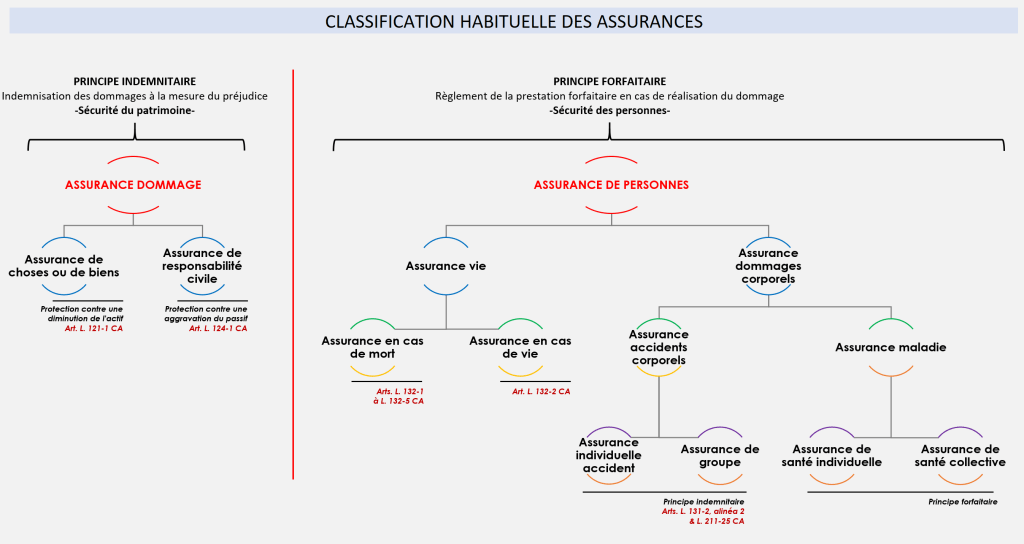
\includegraphics[scale=0.6]{resources/classification-assurances.png}
    \caption{
        \label{classification-assurances} Classification habituelle des assurances - Julien Bourdoiseau
    }
\end{figure}

\newpage
\KOMAoptions{paper=landscape,pagesize}
\section{Fiscalité simplifié en cas de rachat}
\label{appendix:fiscalite-vie}

\begin{figure}[h!]
\centering

\forestset{
    sn edges/.style={
        for tree={
            parent anchor=south, 
            child anchor=north,
            align=center,
            base=bottom,
            where n children=0{tier=word}{}
        }
    },
    background tree/.style={
        for tree={
            text opacity=0.2,
            draw opacity=0.2,
            edge={draw opacity=0.2}
        }
    }
}
\begin{forest}
[Date de souscription,frame, draw
    [Avant le 01/01/1983 
        [\textbf{Exonération}]
    ]
    [Après le 01/01/1983
        [Date de versement, frame, draw
            [Avant le 27 septembre 2017
                [Choix du souscripteur, frame, draw
                    [IR [\textbf{Art. 197} \\ \textbf{CGI}]]
                    [PFL
                        [Ancienneté du contrat, frame, draw
                            [Inférieure à 4 ans [\textbf{35\%}]]
                            [Entre 4 et 8 ans [\textbf{15\%}]]
                            [Supérieure à 8 ans [\textbf{7.5\%}]]
                        ]
                    ]
                ]
            ]
            [Après le 27 septembre 2017
                [Choix du souscripteur, frame, draw
                    [IR [\textbf{Art. 197} \\ \textbf{CGI}]]
                    [PFU
                        [Ancienneté du contrat, frame, draw
                            [Inférieure à 8 ans [\textbf{12.8\%}]]
                            [Supérieure à 8 ans 
                                [Montant des versements, frame, draw
                                    [Inférieur à 150 000 euros [\textbf{7.5\%}]]
                                    [Supérieur à 150 000 euros [\textbf{12.8\%}]]
                                ]
                            ]
                        ]
                    ]
                ]
            ]
        ]
    ]
]
\end{forest}
\caption[]{Taxation simplifiée des produits (hors prélèvements sociaux et abattements)}
\end{figure}


\newpage
\KOMAoptions{paper=landscape,pagesize}
\section{Fiscalité simplifié en cas de décès}
\label{appendix:fiscalite-deces}

\begin{figure}[h!]
\centering

\forestset{
    sn edges/.style={
        for tree={
            parent anchor=south, 
            child anchor=north,
            align=center,
            base=bottom,
            where n children=0{tier=word}{}
        }
    },
    background tree/.style={
        for tree={
            text opacity=0.2,
            draw opacity=0.2,
            edge={draw opacity=0.2}
        }
    }
}
\begin{forest}
[Lien de parenté, frame, draw
    [Conjoint \\ Partenaire de PACS [\textbf{Exonération}]]
    [Non conjoint \\ Non Partenaire de PACS
        [Date de souscription, frame, draw
          [Avant 20 novembre 1991
            [Date de versement des primes, frame, draw 
              [Avant le 13 octobre 1998 [\textbf{Exonération}] ]
              [Après le 13 octobre 1998 [\textbf{990I}] ]
            ]
          ] 
          [Après le 20 novembre 1991 
            [Date de versement des primes, frame, draw 
              [Avant le 13 octobre 1998 
                [Âge de l'assuré \\ au moment du versement, frame, draw 
                  [Versements \\avant 70 ans [\textbf{Exonération}]]
                  [Versements \\après 70 ans [\textbf{757B}]]
                ]
              ]
              [Après le 13 octobre 1998
                [Âge de l'assuré \\ au moment du versement, frame, draw 
                  [Versements \\avant 70 ans [\textbf{990I}]]
                  [Versements \\après 70 ans [\textbf{757B}]]
                ]
              ]
            ] 
          ]
        ]
    ]
]
\end{forest}
\caption[]{Règles d'éligibilité simplifiées aux articles 757B et 990I}
\end{figure}

\newpage
\KOMAoptions{paper=portrait,pagesize}

\end{document}